\documentclass[tikz,border=5pt]{standalone}
\usepackage[T1]{fontenc}
\usepackage{lmodern,amsmath,amssymb}
\usetikzlibrary{arrows.meta,calc,positioning,fit,backgrounds,shapes.geometric,matrix,decorations.pathreplacing,patterns}
\definecolor{ink}{gray}{0.08}
\definecolor{wash}{gray}{0.965}
\definecolor{soft}{gray}{0.45}
\tikzset{box/.style={draw=ink,line width=.65pt,fill=white,align=center,inner sep=4pt,outer sep=0pt,font=\small},flow/.style={draw=ink,line width=.65pt,-{Latex[length=1.8mm,width=1.3mm]},rounded corners=2pt},annotation/.style={font=\scriptsize,text=soft,align=center},groupbox/.style={draw=soft,dashed,line width=.45pt,fill=wash}}
\begin{document}
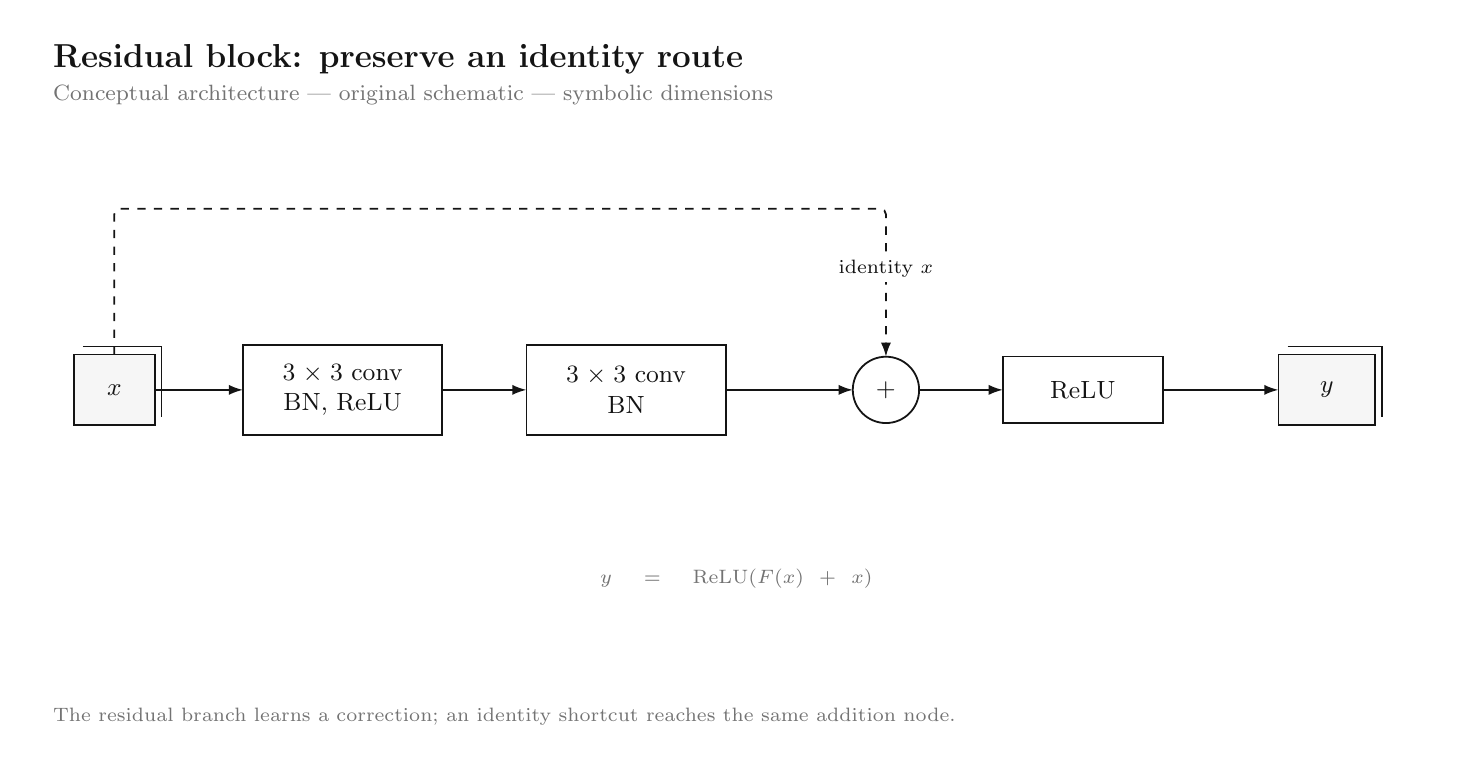
\begin{tikzpicture}[x=1cm,y=-1cm,font=\rmfamily,text=ink]

\path[use as bounding box] (0,0) rectangle (18,9);
\node[anchor=west,font=\large\bfseries] at (.2,.4) {Residual block: preserve an identity route};
\node[anchor=west,font=\footnotesize,text=soft] at (.2,.85) {Conceptual architecture | original schematic | symbolic dimensions};
\begin{pgfonlayer}{background}
\end{pgfonlayer}
\node[box,fill=wash,minimum width=1.0cm,minimum height=0.9cm,text width=0.75cm] (x) at (1.1,4.6) {$x$};
\draw[ink,line width=.4pt] (0.7000000000000001,4.05) -- (1.7000000000000002,4.05) -- (1.7000000000000002,4.95);
\node[box,minimum width=2.5cm,minimum height=1.15cm,text width=2.25cm] (c1) at (4.0,4.6) {$3\times3$ conv\\BN, ReLU};
\node[box,minimum width=2.5cm,minimum height=1.15cm,text width=2.25cm] (c2) at (7.6,4.6) {$3\times3$ conv\\BN};
\node[box,circle,minimum width=0.65cm,minimum height=0.65cm,text width=0.4cm] (sum) at (10.9,4.6) {$+$};
\node[box,minimum width=2cm,minimum height=0.85cm,text width=1.75cm] (relu) at (13.4,4.6) {ReLU};
\node[box,fill=wash,minimum width=1.2cm,minimum height=0.9cm,text width=0.95cm] (y) at (16.5,4.6) {$y$};
\draw[ink,line width=.4pt] (16.0,4.05) -- (17.200000000000003,4.05) -- (17.200000000000003,4.95);
\begin{pgfonlayer}{background}
\draw[flow] (x.east) -- (c1.west);
\draw[flow] (c1.east) -- (c2.west);
\draw[flow] (c2.east) -- (sum.west);
\draw[flow] (sum.east) -- (relu.west);
\draw[flow] (relu.east) -- (y.west);
\draw[flow,dashed] (x.north) -- (1.1,2.3) -- (10.9,2.3) -- (sum.north) node[midway,above,fill=white,inner sep=1.5pt,font=\scriptsize] {identity $x$};
\end{pgfonlayer}
\node[annotation,text width=8cm] at (9,7.0) {$y=\operatorname{ReLU}(F(x)+x)$};
\node[anchor=west,align=left,font=\scriptsize,text=soft,text width=17.6cm] at (.2,8.75) {The residual branch learns a correction; an identity shortcut reaches the same addition node.};
\end{tikzpicture}
\end{document}
